\documentclass[a4paper,12pt]{article}
\usepackage[utf8]{inputenc}
\usepackage[italian]{babel}
\usepackage{amsfonts}
\usepackage{graphicx}
\usepackage{wrapfig}
\usepackage{float}
\usepackage{listings}
\usepackage{color}
\usepackage{subfigure}
\usepackage{ccicons}

\title{Elaborazione di un point cloud e triangolazione con algoritmo Greedy Projection Triangulation}
\author{Davide Pala}
\date{Anno Accademico 2014/2015}
\lstset{ %
language=C++,                % choose the language of the code
keywordstyle=\bfseries\color{green},
commentstyle=\color{magenta},
stringstyle=\color{black},
identifierstyle=\color{blue},
basicstyle=\tiny, % the size of the fonts that are used for the code      
numbers=left,                   % where to put the line-numbers
numberstyle=\footnotesize,      % the size of the fonts that are used for the line-numbers
stepnumber=1,                   % the step between two line-numbers. If it is 1 each line will be numbered
numbersep=5pt,                  % how far the line-numbers are from the code
backgroundcolor=\color{white},  % choose the background color. You must add \usepackage{color}
showtabs=false,                 % show tabs within strings adding particular underscores
frame=lines,           % adds a frame around the code
tabsize=1,          % sets default tabsize to 2 spaces
captionpos=b,           % sets the caption-position to bottom
breaklines=true,        % sets automatic line breaking
breakatwhitespace=false,    % sets if automatic breaks should only happen at whitespace
showstringspaces=false,
escapeinside={\%*}{*)}          % if you want to add a comment within your code
}

\begin{document}
\maketitle
\begin{figure}[H]
\centering

\includegraphics[width=13cm]{pics/logo_diana.jpg}
\end{figure}
\
\
\
\begin{center}
\small{distribuito secondo la licenza Creative Commons: \ccbyncsa}
\end{center}

\clearpage
\tableofcontents
\clearpage
\section{Introduzione}
	\subsection{Team DIANA}
	Il team Diana è un gruppo studentesco del Politecnico di Torino che si occupa di
	robotica spaziale, nato per rappresentare l'ateneo all'interno del progetto 
	AMALIA\footnote{http://www.amalia-teamitalia.it/}. 
	L'attività del team è dedita principalmente allo sviluppo di un rover lunare 
	in tutte le sue funzionalità. 
	Il rover è dotato, allo stato attuale, di un sistema di acquisizione di immagini 
	composto da due camere Black-and-White di Point 
	Gray\footnote{http://team-diana.github.io/en/\#!pages/blackfly\_bw\_poe\_gige\_hardware.md} 
	e da un sensore Mesa SR4500 ToF	camera\footnote{http://team-diana.github.io/en/\#!pages/sr4500.md}.
	Questa strumentazione permette al sistema di effettuare delle riprese in cui vengono acquisiti dei 
	Point Cloud, insiemi di punti dello spazio tridimensionale che descrivono la scena ripresa.
	
	\subsection{Obiettivi e descrizione del progetto}
	Lo scopo del programma è generare una mesh poligonale effettuando la triangolazione di un point cloud.
	Il programma acquisice il nome del file contenente il point cloud e il nome del file di output da linea di comando,
	i punti vengono letti dal file e processati da una serie di algoritmi di filtraggio. 
	Successivamente viene applicato lo smoothing delle superfici, durante il quale viene effettuato anche il calcolo delle
	normali, in ultimo l'algoritmo di ricostruzione dei triangoli elabora il point cloud, la mesh così generata viene quindi
	scritta sul file di output.  
	Il software è scritto in C++, per lo sviluppo è stato utilizzato l'IDE Qt Creator\footnote{http://wiki.qt.io/Qt\_Creator},
	mentre per le strutture dati e gli algoritmi per il processing del point cloud è stata utilizzata la libreria
	pcl\footnote{http://pointclouds.org/about/}. 	
	
\clearpage
\section{Il programma}
	\subsection{Approccio Object Oriented}
	Il programma è stato sviluppato seguendo l'approccio della programmazione orientata agli oggetti: 
	una facade class, PointCloudTriangulation, espone al main le funzioni per la lettura  e l'elaborazione del point cloud
	e per la gestione dei filtri, che sono immagazinati internamente con una mappa che associa una stringa, 
	il nome del filtro, ad un puntatore generico a PointCloudFilter.	
	La classe espone anche le funzioni per effettuare la triangolazione e per salvarne il risultato su file, sono
	inoltre definiti i valori di default dei parametri della triangolazione.
	\begin{figure}[H]	
	\begin{lstlisting}	
	#define PARAM_SEARCH_RADIUS 0
	#define PARAM_MULTIPLIER 1
	#define PARAM_MAX_NEAREST_NEIGHBORS 2
	#define PARAM_MAX_SURFACE_ANGLE 3
	#define PARAM_MIN_ANGLE 4
	#define PARAM_MAX_ANGLE 5
	#define PARAM_NORMAL_CONSISTENCY 6
	
	#define DEFAULT_SEARCH_RADIUS 0.025
	#define DEFAULT_MULTIPLIER 2.5
	#define DEFAULT_MAX_NEAREST_NEIGHBORS 100
	#define DEFAULT_MAX_SURFACE_ANGLE M_PI/4 
	#define DEFAULT_MIN_ANGLE M_PI/18  //10
	#define DEFAULT_MAX_ANGLE 2*M_PI/3 //120
	#define DEFAULT_NORMAL_CONSISTENCY true
	
	class PointCloudTriangulation
	{
	private:
    	pcl::PointCloud<pcl::PointXYZ>::Ptr cloud;
    	pcl::PointCloud<pcl::PointNormal>::Ptr normalCloud;
    	pcl::GreedyProjectionTriangulation<pcl::PointNormal> gp3;
    	pcl::PolygonMesh triangles;
    	std::map<std::string, PointCloudFilter* > algorithms;
    
	public:
   		PointCloudTriangulation(pcl::PointCloud<pcl::PointNormal>::Ptr);
    	PointCloudTriangulation(std::string);
    	PointCloudTriangulation();

	    void addFilter(std::string, PointCloudFilter*);
    	void applyFilter(std::string);
    	void loadCloudFromFile(std::string);
    	void surfaceSmoothing();
    	void reconstruct(); //apply greedy projection triangulation
    	void saveTriangulation(std::string);
    	PointCloudFilter* getFilter(std::string);
    	pcl::PointCloud<pcl::PointNormal>::Ptr getCloud();
    	pcl::PolygonMesh getTriangulation();    
	};	
	\end{lstlisting}
	\label{fig:PointCloudTriangulation}
	\caption{la classe PointCloudTriangulation}
	\end{figure}
	\clearpage
	
	PointCloudFilter è una classe puramente virtuale realizzata come interfaccia per la gestione dei filtri,
	dichiara soltanto 3 metodi utili per applicare l'algoritmo e settarne o leggerne i parametri.
	I parametri sono identificati da delle costanti numeriche e sono trattati come dei double.
	L'effettiva implementazione dei filtri è realizzata con 2 sottoclassi di PointCloudFilter: PCVoxelGridFilter
	e PCStatisticalOutlierRemoval. 
	\begin{figure}[H]
	\begin{lstlisting}
	class PointCloudFilter
	{
	public:
    	virtual void apply(pcl::PointCloud<pcl::PointNormal>::Ptr) = 0;
    	virtual void setParameter(int, double) = 0;
    	virtual double getParameter(int) = 0;
	};
	\end{lstlisting}
	\label{fig:PointCloudFilter}
	\caption{la classe PointCloudFilter}
	\end{figure}
	\clearpage
	\subsection{Il main}
	Grazie all'utilizzo della facade class e il main del programma risulta particolarmente conciso.
	Dopo il controllo degli argomenti da linea di comando, viene allocata un'istanza della facade class, 
	triangulation, quindi si passa alla lettura del file contenente il point cloud. 
	Due puntatori generici a PointCloudFilter vengono allocati come oggetti di tipo PCVoxelGridFilter e
	PCStatisticalOutlierRemoval e aggiunti a all'oggetto triangulation assegnandogli un identificatore di
	tipo string. I due filtri sono quindi applicati sul point cloud e, dopo il surface smoothing, 
	$triangulation\rightarrow reconstruct()$ genera la mesh poligonale, che viene quindi salvata sul file di output.
	\begin{figure}[H]
	\begin{lstlisting}
int main(int argc,char **argv)
{
    help(argc, argv); // check command line args
    
    PointCloudTriangulation *triangulation = new PointCloudTriangulation();

    triangulation->loadCloudFromFile(argv[1]); // read cloud from pcd file

    PointCloudFilter* voxel_grid_filter = new PCVoxelGridFilter();
    PointCloudFilter* gaussian_noise_filter = new PCStatisticalOutlierRemoval();

    triangulation->addFilter("voxel grid filter", voxel_grid_filter);
    triangulation->addFilter("gaussian noise filter", gaussian_noise_filter);

    triangulation->applyFilter("voxel grid filter");
    triangulation->applyFilter("gaussian noise filter");

    triangulation->surfaceSmoothing();
    triangulation->reconstruct();

    triangulation->saveTriangulation(argv[2]);

    return 0;
}
	\end{lstlisting}
	\label{fig:main}
	\caption{il main del programmga}	
	\end{figure}
	\clearpage
	\subsection{I filtri}
		\subsubsection{Voxel Grid Filter}
		Il tempo di calcolo è stato il primo problema incontrato durante lo sviluppo; infatti
		il tempo necessario per l'esecuzione di surface smoothin e triangolazione su un point cloud di 460400 punti è
		di circa 2 minuti, mentre applicando tutte le elaborazioni dopo il downsample,
		il tempo di esecuzione è sceso al di sotto dei 10 secondi, spesi perlopiù nella fase di lettura del file.
		\begin{figure}[H]
    	\centering
    	\subfigure[]{
        	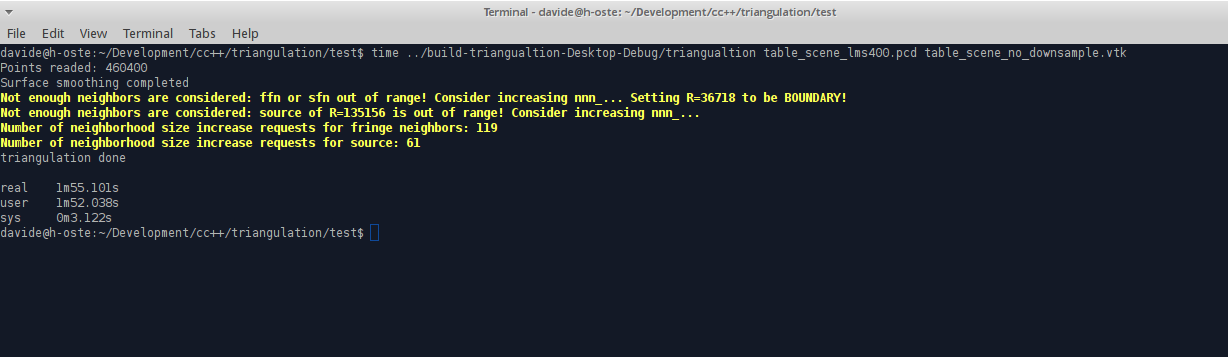
\includegraphics[width=13cm]{pics/no_downsample_time.png}
        	\label{fig:no_downsample_time}
    	}
    	\subfigure[]{
        	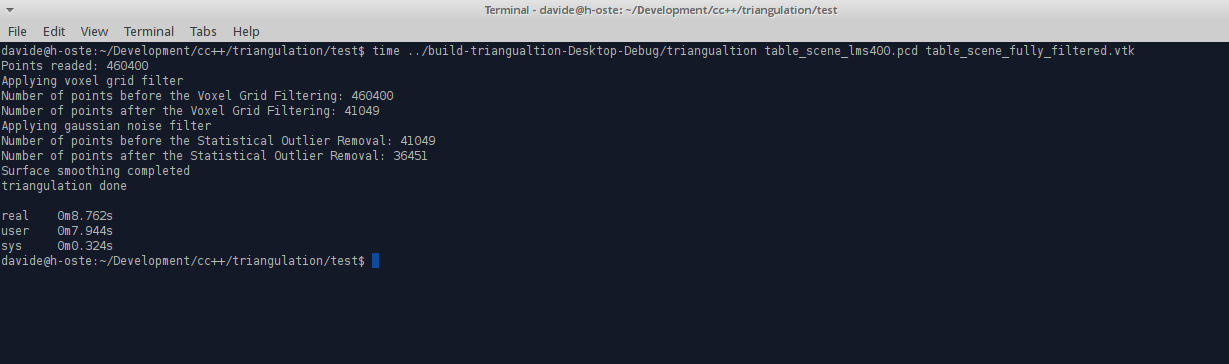
\includegraphics[width=13cm]{pics/full_time.png}
        	\label{fig:full_time}
    	}
    	\caption{confronto fra i tempi di esecuzione con e senza downsample}
    	\label{fig:time_comparison}
		\end{figure}		
		Per realizzare il downsample del point cloud è stato utilizzato l'algoritmo di voxel grid filtering.
		Questo algoritmo funziona suddividendo lo spazio in una griglia di voxel, piccole unità di volume, tutti i punti
		all'interno di un voxel vengono approssimati dal loro baricentro.
		Il filtro ha tre parametri fondamentali che sono la lunghezza degli spigoli del voxel lungo i 3 assi cartesiani.
		\begin{figure}[H]
		\begin{lstlisting}
#define DEFAULT_LEAF_SIZE 0.01f
#define PARAM_LEAF_SIZE_X 0 //"leaf size x"
#define PARAM_LEAF_SIZE_Y 1 //"leaf size y"
#define PARAM_LEAF_SIZE_Z 2 //"leaf size z"

class PCVoxelGridFilter : public PointCloudFilter
{
public:
    PCVoxelGridFilter();
    void apply(pcl::PointCloud<pcl::PointXYZ>::Ptr cloud);
    //void setParameter(int, std::string);
    void setParameter(int, double);
    double getParameter(int);
    bool isValidParam(int);
private:
    pcl::VoxelGrid< pcl::PointXYZ> voxel_grid_filter;
    std::map<int, double> params;
};
		\end{lstlisting}
		\caption{la classe PCVoxelGridFilter}
		\label{pcvoxelgridfilter}		
		\end{figure}	
		La classe che realizza il filtro è PCVoxelGridFilter ed implementa l'interfaccia PointCloudFilter, il metodo 
		$apply()$ imposta i parametri ed applica il filtro, come dimensione di default per i lati del voxel è stata scelta 
		0.01, che dovrebbe corrispondere a cubi di spigolo un centimetro, con questa configurazione il numero di punti
		del point cloud di test viene ridotto da 460400 a 41049, un fattore di circa 11.
		\begin{figure}[H]
		\begin{lstlisting}
void PCVoxelGridFilter::apply(pcl::PointCloud<pcl::PointXYZ>::Ptr cloud)
{
    std::cout<<"Number of points before the Voxel Grid Filtering: "<<cloud->width*cloud->height<<std::endl;
    voxel_grid_filter.setInputCloud(cloud);
    voxel_grid_filter.setLeafSize((float)params[PARAM_LEAF_SIZE_X],
                                  (float)params[PARAM_LEAF_SIZE_Y], 
                                  (float)params[PARAM_LEAF_SIZE_Z]);
    voxel_grid_filter.filter(*cloud);
    std::cout<<"Number of points after the Voxel Grid Filtering: "<<cloud->width*cloud->height<<std::endl;
}
		\end{lstlisting}
		\caption{il metodo $apply()$ della classe PCVoxelGridFilter}
		\label{apply_voxel}
		\end{figure}		
		\clearpage	 
		\subsubsection{Statistical Outlier Removal}
		Il secondo stadio di filtraggio si occupa di attenuare e rimuovere il rumore del cloud, infatti, durante la 
		cattura, i sensori rilevano punti errati, spesso a causa di riflessi o errori di misura, questi errori complicano
		poi le elaborazioni successive e rischiano di condurre a risultati sbagliati, per esempio nel calcolo delle normali.
		
		Anche in questo caso la classe che implementa il filtro, PCStatisticalOutlierRemoval, è una sottoclasse di
		PointCloudFilter e implementa quindi i soliti metodi $getParameter()$, $setParameter()$ ed $apply()$.
		\begin{figure}[H]
		\begin{lstlisting}
//number of point to use for mean distance estimation
#define PARAM_MEAN_K 0 //"mean k"
#define PARAM_STD_DEV_MUL_TH 1 //"standard deviation multipilier threashold"

// default values
#define DEFAULT_MEAN_K 50
#define DEFAULT_STD_DEV_MUL_TH 0.1

class PCStatisticalOutlierRemoval : public PointCloudFilter
{
public:

    PCStatisticalOutlierRemoval();
    void apply(pcl::PointCloud<pcl::PointXYZ>::Ptr cloud);
    void setParameter(int, double);
    double getParameter(int);

private:
    std::map<int, double> parameters;
    pcl::StatisticalOutlierRemoval<pcl::PointXYZ> sor;

};
		\end{lstlisting}
		\caption{la classe PCStatisticalOutlierRemoval}
		\label{pcstatisticaloutlierremoval}
		\end{figure}
		
		Il principio di funzionamento dell'algoritmo si basa sul valutare punto per punto la distanza media da tutti i suoi $n$
		vicini, la distribuzione risultante viene considerata come una gaussiana con una media e una deviazione standard
		$\sigma$, tutti i punti appartenenti al vicinato la cui distanza supera il valore $m\times\sigma$ sono considerati
		outlier e rimossi dall'insieme. 
		I parametri del filtro sono il numero $n$ di vicini da considerare e il moltiplicatore $m$ della deviazione standard, 
		i valori scelti come default sono $n=50$ e $m=1.0$, il filtro rimuove quindi tutti i punti la cui
		distanza supera un $\sigma$.
		\begin{figure}
		\begin{lstlisting}
void PCStatisticalOutlierRemoval::apply(pcl::PointCloud<pcl::PointXYZ>::Ptr cloud){
    std::cout<<"Number of points before the Statistical Outlier Removal: "<<cloud->width*cloud->height<<std::endl;
    sor.setInputCloud (cloud);
    sor.setMeanK ((int)parameters[PARAM_MEAN_K]);
    sor.setStddevMulThresh ((float)parameters[PARAM_STD_DEV_MUL_TH]);
    sor.filter (*cloud);
    std::cout<<"Number of points after the Statistical Outlier Removal: "<<cloud->width*cloud->height<<std::endl;
}
		\end{lstlisting}
		\caption{il metodo $apply()$ della classe PCStatisticalOutlierRemoval}
		\label{apply_sor}
		\end{figure}
		
		\begin{figure}[H]
    	\centering
    	\subfigure[]{
        	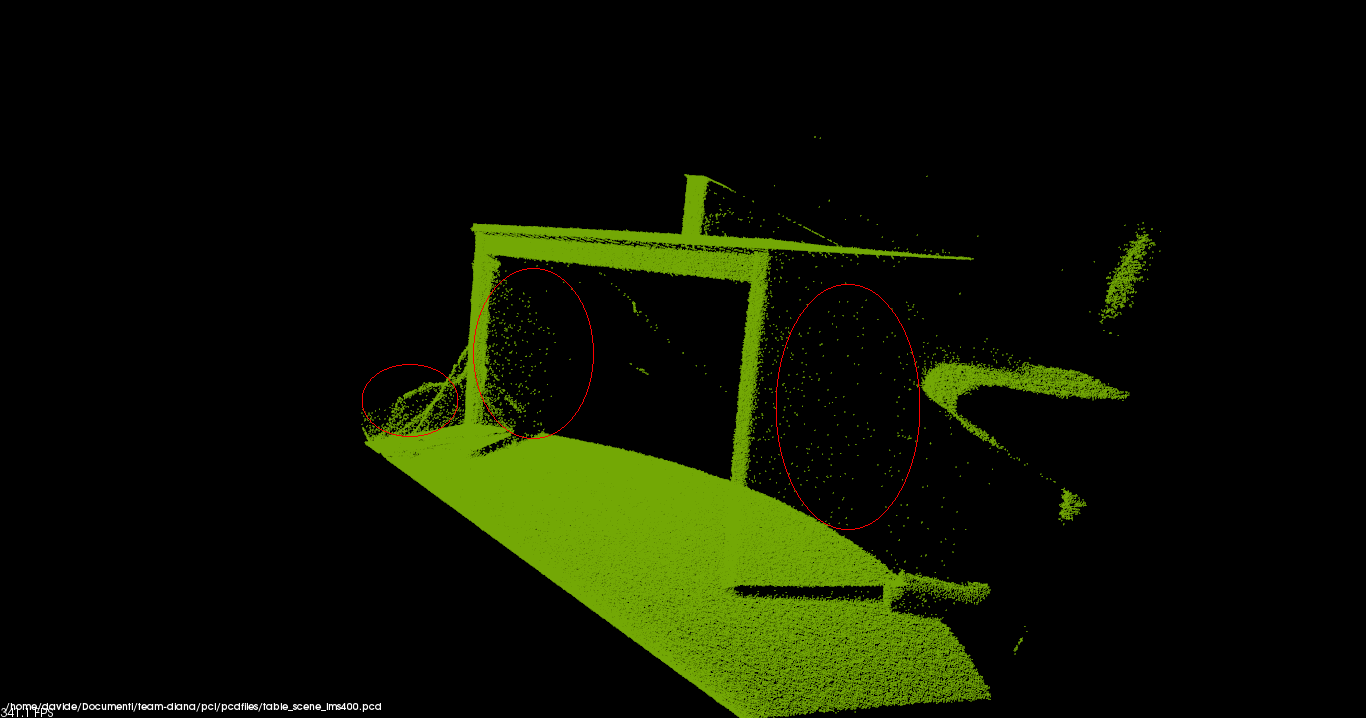
\includegraphics[width=13cm]{pics/table_scene_noise3.png}
        	\label{fig:noise}
    	}
    	\subfigure[]{
        	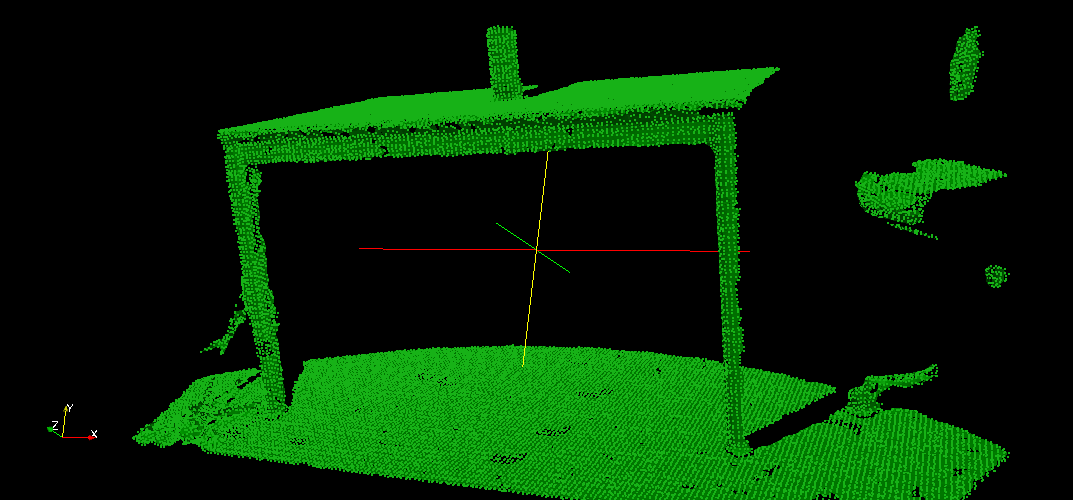
\includegraphics[width=13cm]{pics/table_scene_mesh.png}
        	\label{fig:mesh}
    	}
    	\caption{il point cloud non filtrato (a) e la mesh (b)}
    	\label{fig:noise_comparison}
		\end{figure}
	\clearpage
	\subsection{Surface Smoothing}
	L'algoritmo di surface smoothing "mooving least squares" si occupa di fare una ricostruzione delle superfici basata su 
	un resample del cloud e sul'iterpolazione polinomiale, questa elaborazione dovrebbe contibuire a ridurre il rumore e i
	piccoli difetti del data set, inoltre l'algoritmo di triangolazione ha un risultato migliore se effettuato su superfici
	regolari. Il parametro fondamentale di questo algoritmo è il raggio di ricerca, il raggio della sfera usata per cercare i
	vicini su cui effettuare il fit polinomiale, per i restanti parametri è stato lasciato il valore di default specificato
	dalla libreria.
	\begin{figure}[H]
	\begin{lstlisting}
	void PointCloudTriangulation::surfaceSmoothing(){
    	pcl::search::KdTree<pcl::PointXYZ>::Ptr tree(new pcl::search::KdTree<pcl::PointXYZ>());
    	pcl::MovingLeastSquares<pcl::PointXYZ, pcl::PointNormal> mls;

    	mls.setComputeNormals(true);

    	mls.setInputCloud(cloud);
    	mls.setPolynomialFit(true);
    	mls.setSearchMethod(tree);
    	mls.setSearchRadius(0.03);

    	mls.process(*normalCloud);
    	std::cout<<"Surface smoothing compleated"<<std::endl;
	}
	\end{lstlisting}
	\caption{$surfaceSmoothing()$ nella classe PointCloudTriangulation}
	\label{mls}
	\end{figure}	 
		\subsubsection{Normal Estimation}
		L'algoritmo di surface smoothing si occupa anche di effettuare il calcolo delle normali, nelle fasi 
		iniziali dello sviluppo per il surface smoothing era stato utilizzato lo stesso approccio adottato con i filtri,
		le normali venivano quindi calcolate immediatamente dopo la lettura dei dati dal file, questo per avere una
		coerenza sui tipi di dato su cui operano i filtri, ciò comportava un tempo di elaborazione più lungo 
		e una maggiore complessita del codice che doveva gestire anche i parametri dell'algoritmo di normal estimation.
	\clearpage
	\subsection{Greedy Projection Triangulation}
	Il core del programma consiste nella generazione una mesh poligonale a partire da un point cloud con le normali.
	Per lo scopo viene utilizzato l'algoritmo di greedy projection triangulation, questo metodo si basa sulla triangolazione
	locale dei vicini di un punto, che vengono proiettati lungo la normale del punto stesso, i punti non ancora connessi
	vengono collegati. Il metodo ha numerosi parametri: "maximum nearest neighbors" specifica il numero massimo di vicini,
	il "multiplier" specifica la massima distanza per la quale un punto può essere considerato un vicino, relativa al punto
	a distanza minima, il "search radius" è il raggio di ricerca per i vicini e limita la dimensione massima dei lati dei 
	triangoli, "minimum angle" e "maximum angle" definiscono il massimo e il minimo valore per gli angoli all'interno dei 
	triangoli, "maximum surface angle" specifica il massimo angolo di deviazione tra la normale di un punto e quella di
	un suo vicino affinché questo possa essere considerato per la triangolazione.
	\begin{figure}[H]
	\begin{lstlisting}
	void PointCloudTriangulation::reconstruct(){
    	// Create search tree*
    	pcl::search::KdTree<pcl::PointNormal>::Ptr tree (new pcl::search::KdTree<pcl::PointNormal>);
    	tree->setInputCloud (normalCloud);
	
    	// Set the maximum distance between connected points (maximum edge length)
    	gp3.setSearchRadius (DEFAULT_SEARCH_RADIUS);
	
    	// Set typical values for the parameters
    	gp3.setMu (DEFAULT_MULTIPLIER); // 2.5
    	gp3.setMaximumNearestNeighbors (DEFAULT_MAX_NEAREST_NEIGHBORS); // 100
    	gp3.setMaximumSurfaceAngle(DEFAULT_MAX_SURFACE_ANGLE); // 45 degrees
	    gp3.setMinimumAngle(DEFAULT_MIN_ANGLE); // 10 degrees
    	gp3.setMaximumAngle(DEFAULT_MAX_ANGLE); // 120 degrees
    	gp3.setNormalConsistency(true);

    	// Get result
    	gp3.setInputCloud (normalCloud);
    	gp3.setSearchMethod (tree);
    	gp3.reconstruct (triangles);
    	std::cout<<"triangulation done"<<std::endl;
	}
	\end{lstlisting}
	\caption{il metodo $reconstruct()$ della classe PointCloudTriangulation}
	\label{reconstruct}
	\end{figure}
	\clearpage
	
	
\section{Considerazioni e Sviluppi futuri}
Questo lavoro ha richiesto molto tempo, sopratutto per la ricerca e la comprensione degli algoritmi e dei loro 
parametri, tuttavia non è da intendersi come un progetto concluso:
sono possibili numerosi sviluppi e modifiche e il software è in continuo aggiornamento, è inoltre necessario 
efettuare dei test per affinare i valori dei parametri e per adattarli ai dati acquisiti dal rover.
	\subsection{Sviluppi futuri}
	La prima necessità che emerge dall'utilizzo del programma è quella di una più facile gestione dei parametri, 
	infatti, seppure l'approccio object oriented ne facilita l'utilizzo, la configurazione dei valori è statica e
	bisogna ricompilare il programma ogni volta che si effettua una modifica, per questo motivo una configurazione
	con lettura da file sembra la via più efficace. Per un eventuale file di configurazione stiamo valutando, 
	al momento, due formati: xml e YALM\footnote{http://yaml.org/}.
	
	Il passo successivo dello sviluppo sarà quello dell'integrazione con ROS\footnote{http://www.ros.org/} e della creazione di un nodo 
	in grado di ricevere i point cloud rilevati dal rover ed elaborarli, enventualmente in tempo reale, con la possibilità di 
	effettuare tutta la catena per la triangolazione, o magari di effettuare solo un live filtering in modo da pulire i 
	dati per altre applicazioni.
	\subsection{Conclusioni}
	Questo lavoro, e in generale tutta l'esperienza con il team DIANA, mi ha permesso di esplorare, anche se superficialmente, 
	il mondo della computer vision, ho acquisito inoltre una maggiore familiarità con il linguaggio C++, con le librerie 
	PCL e tutti gli strumenti di sviluppo, è stato anche un'ottima occasione per poter applicare le conoscenze apprese durante 
	i corsi seguiti in questi anni per la soluzione di problemi pratici.
	   
\end{document}
